\section{测序技术}
\begin{frame}
  \frametitle{基因组学 | 测序 | 简介}
  \begin{block}{DNA测序}
DNA测序(DNA sequencing)是指分析特定DNA片段的碱基序列,也就是腺嘌呤(A)、胸腺嘧啶(T)、胞嘧啶(C)与鸟嘌呤(G)的排列方式。
  \end{block}
  \pause
  \begin{block}{RNA测序}
RNA测序则通常将RNA提取后,反转录为DNA后使用DNA测序的方法进行测序。
  \end{block}
\end{frame}

\subsection{第一代测序技术}
\begin{frame}
  \frametitle{基因组学 | 测序 | 第一代 | 简介}
   \begin{itemize}
     \item 1975年,弗雷德里克·桑格和艾伦·库尔森(Alan Coulson),“加减测序法技术”;改进后为链终止法(chain termination method),即桑格测序法
     \item 1977年,哈佛大学的沃尔特·吉尔伯特和艾伦·马克萨姆(Allan Maxam),马克萨姆-吉尔伯特测序(Maxam-Gilbert法,又称化学测序法)
   \end{itemize} 
\end{frame}

\begin{frame}
  \frametitle{基因组学 | 测序 | 第一代 | 化学测序法}
  \begin{block}{化学测序法}
马克萨姆-吉尔伯特测序(Maxam-Gilbert sequencing)是一项由阿伦·马克萨姆与沃尔特·吉尔伯特于1976~1977年间开发的DNA测序方法。此项方法基于:对核碱基特异性地进行局部化学改性,接下来在改性核苷酸毗邻的位点处DNA骨架发生断裂。\\
\vspace{1em}
最初的桑格法须要在每次读序之前克隆得到单链DNA产物,因此马克萨姆-吉尔伯特测序法发表后迅速得到了推广,因为被纯化的DNA可被直接使用。然而,随着链终止法的改良,马克萨姆-吉尔伯特测序逐渐失宠,这是由于:技术复杂性阻碍其成为标准分子生物学套装使用、大量使用危险药品以及难于扩大规模。
  \end{block}
\end{frame}

\begin{frame}
  \frametitle{基因组学 | 测序 | 第一代 | 化学测序法}
  \begin{figure}
    \centering
    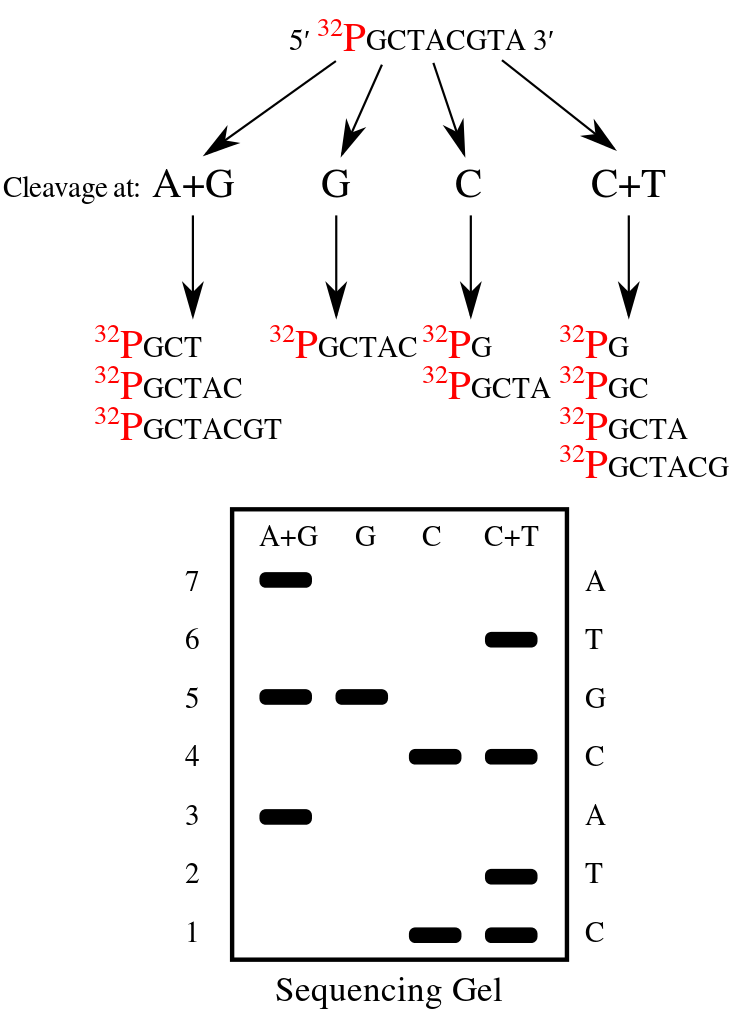
\includegraphics[width=0.48\textwidth]{c2.genomics/sequencing.mg.01.png}
  \end{figure}
\end{frame}

\begin{frame}
  \frametitle{基因组学 | 测序 | 第一代 | 桑格测序法}
  \begin{block}{桑格测序法}
Sanger(桑格)双脱氧链终止法是弗雷德里克·桑格(Frederick Sanger)于1975年发明的。测序过程需要先做一个聚合酶连锁反应(PCR)。PCR过程中,双脱氧核糖核苷酸可能随机的被加入到正在合成中的DNA片段里。由于双脱氧核糖核苷酸少了一个氧原子,一旦它被加入到DNA链上,这个DNA链就不能继续增加长度。最终的结果是获得所有可能获得的、不同长度的DNA片段。\\
\vspace{1em}
目前最普遍最先进的方法,是将双脱氧核糖核苷酸进行不同荧光标记。将PCR反应获得的总DNA通过毛细管电泳分离,跑到最末端的DNA就可以在激光的作用下发出荧光。由于ddATP, ddGTP, ddCTP, ddTTP(4种双脱氧核糖核苷酸)荧光标记不同,计算机可以自动根据颜色判断该位置上碱基究竟是A,T,G,C中的哪一个。 
  \end{block}
\end{frame}

\begin{frame}
  \frametitle{基因组学 | 测序 | 第一代 | 桑格测序法}
  \begin{block}{原理}
双脱氧链终止法采用DNA复制原理。Sanger测序反应体系中包括目标DNA片断、脱氧三磷酸核苷酸(dNTP)、双脱氧三磷酸核苷酸(ddNTP)、测序引物及DNA聚合酶等。 测序反应的核心就是其使用的ddNTP:由于缺少3'-OH基团,不具有与另一个dNTP连接形成磷酸二酯键的能力,这些ddNTP可用来中止DNA链的延伸。此外,这些ddNTP上连接有放射性同位素或荧光标记基团,因此可以被自动化的仪器或凝胶成像系统所检测到。
  \end{block}
\end{frame}

\begin{frame}
  \frametitle{基因组学 | 测序 | 第一代 | 桑格测序法}
  \begin{block}{优势}
    \begin{itemize}
      \item 最长可测定600-1000bp的DNA片断
      \item 对重复序列和多聚序列的处理较好
      \item 序列准确性高
      \item 测序的“黄金标准”
    \end{itemize}
  \end{block}
  \pause
  \begin{block}{缺点}
    \begin{itemize}
      \item 通量较低(在24h内可测定的DNA分子数一般不超过10,000个)
      \item 每碱基测序成本较高
      \item 不适合大规模平行测序
    \end{itemize}
  \end{block}
\end{frame}

\begin{frame}
  \frametitle{基因组学 | 测序 | 第一代 | 桑格测序法}
  \begin{figure}
    \centering
    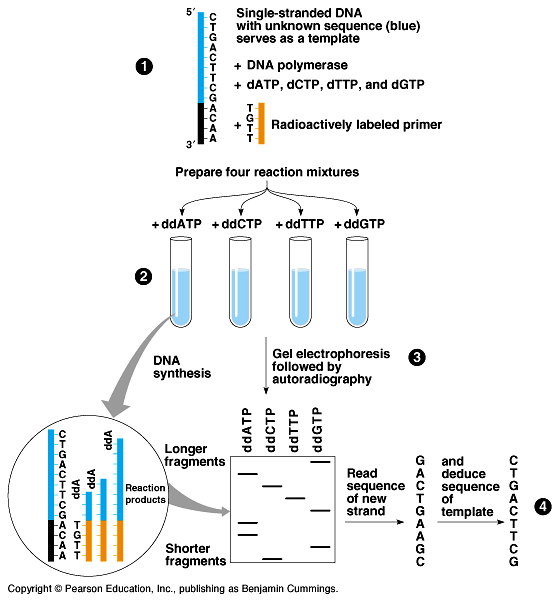
\includegraphics[width=0.6\textwidth]{c2.genomics/sequencing.sanger.01.png}
  \end{figure}
\end{frame}

\begin{frame}
  \frametitle{基因组学 | 测序 | 第一代 | 桑格测序法}
  \begin{figure}
    \centering
    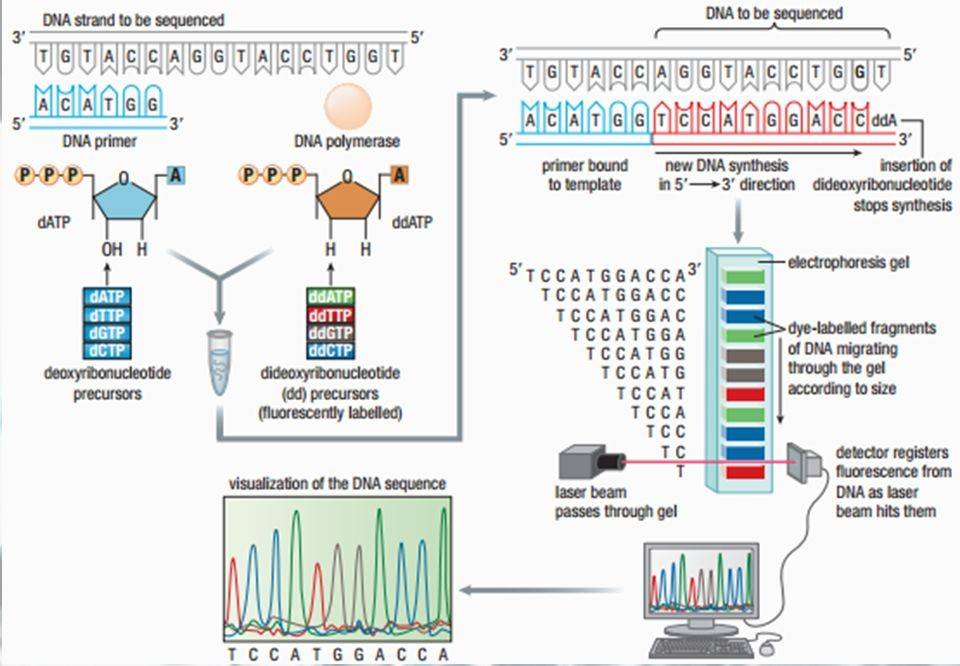
\includegraphics[width=0.9\textwidth]{c2.genomics/sequencing.sanger.04.jpg}
  \end{figure}
\end{frame}

\subsection{第二代测序技术}
\begin{frame}[label=current]
  \frametitle{基因组学 | 测序 | 第二代 | 简介}
  \begin{itemize}
    \item 1996年,波尔·尼伦和穆斯塔法·罗纳吉,焦磷酸测序(Pyrosequencing)
    \item 2004年,454生命科学公司(现为Roche诊断公司的一部分),第一台商品化新一代测序仪——基因组测序仪20
    \item 2006年12月,454生命科学公司,第二代仪器——基因组测序仪FLX(GS FLX)
  \end{itemize}
  \pause
  \begin{itemize}
    \item 
  \end{itemize}
  \pause
  \begin{itemize}
    \item 
  \end{itemize}
\end{frame}

\begin{frame}
  \frametitle{基因组学 | 测序 | 第二代 | 焦磷酸测序}
  \begin{block}{焦磷酸测序}
焦磷酸测序(pyrosequencing)是一种基于聚合原理的DNA测序方法,它依赖于核苷酸掺入中焦磷酸盐的释放,而非双脱氧核苷三磷酸参与的链终止反应。\\
\vspace{1em}
Pyrosequencing技术是由4种酶催化的同一反应体系中的酶级联化学发光反应。在每一轮测序中,只加入一种dNTP,若该dNTP与模板配对,聚合酶就可以将其掺入到引物链中并释放出等摩尔数的焦磷酸基团(PPi)。PPi可最终转化为可见光信号,并由PyrogramTM转化为一个峰值。每个峰值的高度与反应中掺入的核苷酸数目成正比。然后加入下一种dNTP,继续DNA链的合成。
  \end{block}
\end{frame}

\begin{frame}
  \frametitle{基因组学 | 测序 | 第二代 | 焦磷酸测序}
  \begin{block}{emPCR}
emPCR主要通过将水相PCR溶液(包含引物、聚合酶、核苷酸和待扩增DNA)与油混合,创建一种微小的悬浮水滴乳液。每个液滴都作为其自身PCR的“反应器”,从而创造了平行反应中的多个独立反应。\\
\vspace{1em}
emPCR(emulsion PCR)技术利用油包水(water-in-oil)结构作为PCR反应的微反应器,进行PCR扩增。emPCR最大的特点是可以形成数目庞大的独立反应空间以进行PCR扩增。其关键技术是“注水到油”,基本过程是在PCR反应前,将包含PCR所需反应成分的水溶液注入到高速旋转的油相表面,水溶液瞬间形成数以万计个被油相包裹的小液滴。这些小液滴就形成了PCR反应空间。
  \end{block}
\end{frame}

% \begin{frame}
%   \frametitle{基因组学 | 测序 | 第二代 | 焦磷酸测序}
%   \begin{figure}
%     \centering
%     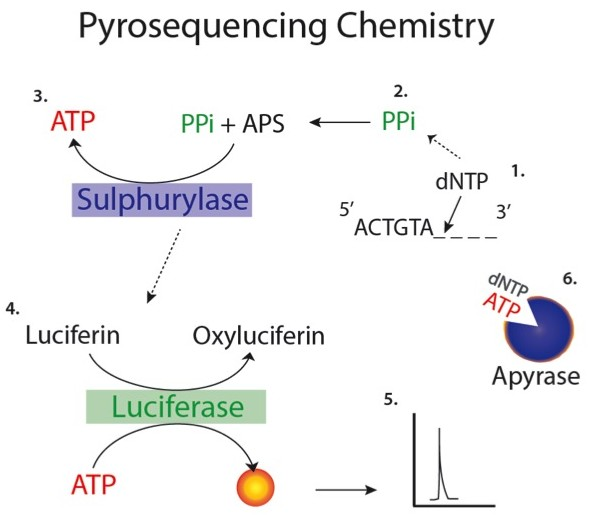
\includegraphics[width=0.7\textwidth]{c2.genomics/sequencing.pyro.01.jpg}
%   \end{figure}
% \end{frame}

\begin{frame}
  \frametitle{基因组学 | 测序 | 第二代 | 焦磷酸测序}
  \begin{figure}
    \centering
    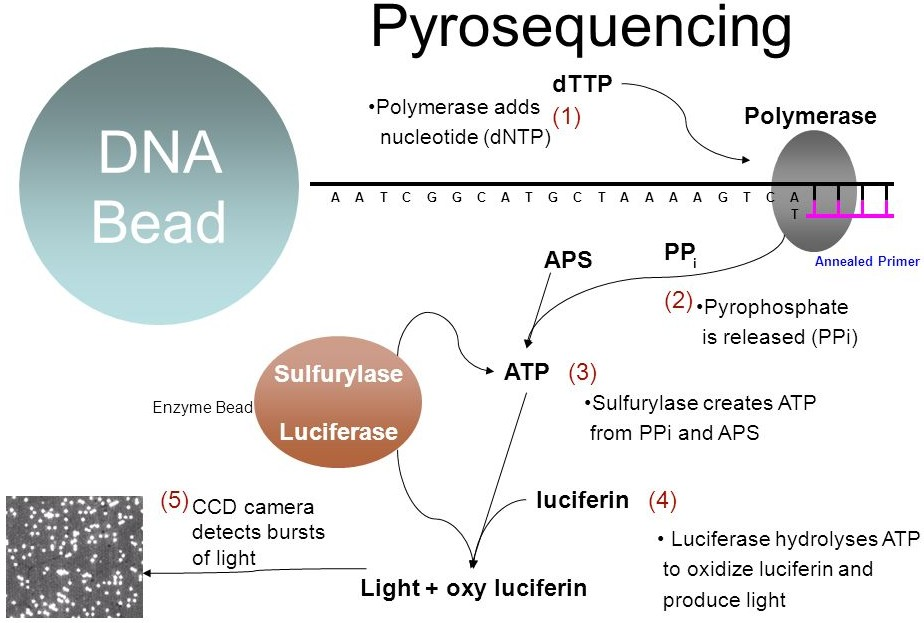
\includegraphics[width=0.9\textwidth]{c2.genomics/sequencing.pyro.02.jpg}
  \end{figure}
\end{frame}

\begin{frame}
  \frametitle{基因组学 | 测序 | 第二代 | 焦磷酸测序}
  \begin{figure}
    \centering
    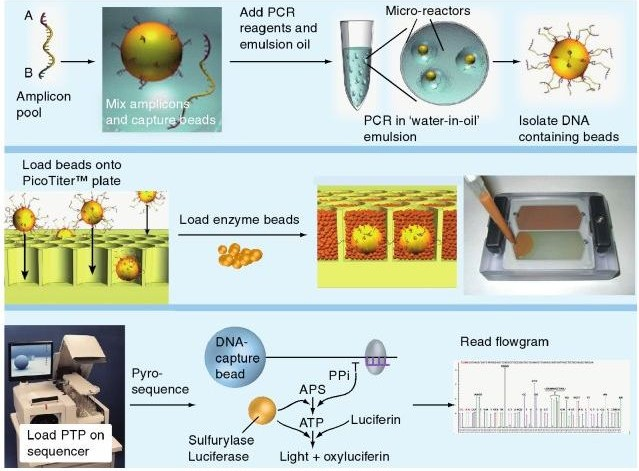
\includegraphics[width=0.9\textwidth]{c2.genomics/sequencing.454.01.jpg}
  \end{figure}
\end{frame}

\begin{frame}
  \frametitle{基因组学 | 测序 | 第二代 | 边合成边测序}
  \begin{block}{边合成边测序}
边合成边测序(Sequencing by Synthesis,SBS):以DNA单链为模板,在合成互补链的时候,利用带荧光标记的dNTP发出不同的荧光来确定碱基类型。
  \end{block}
  \pause
  \begin{block}{桥式扩增}
桥式扩增(Bridge Amplification):随机打断的单链DNA片段通过两端接头与寡核苷酸的互补固定在芯片表面,形成桥形结构,之后以寡核苷酸为引物进行PCR扩增,得到单克隆的DNA簇群。
  \end{block}
\end{frame}

\begin{frame}
  \frametitle{基因组学 | 测序 | 第二代 | 边合成边测序}
  \begin{figure}
    \centering
    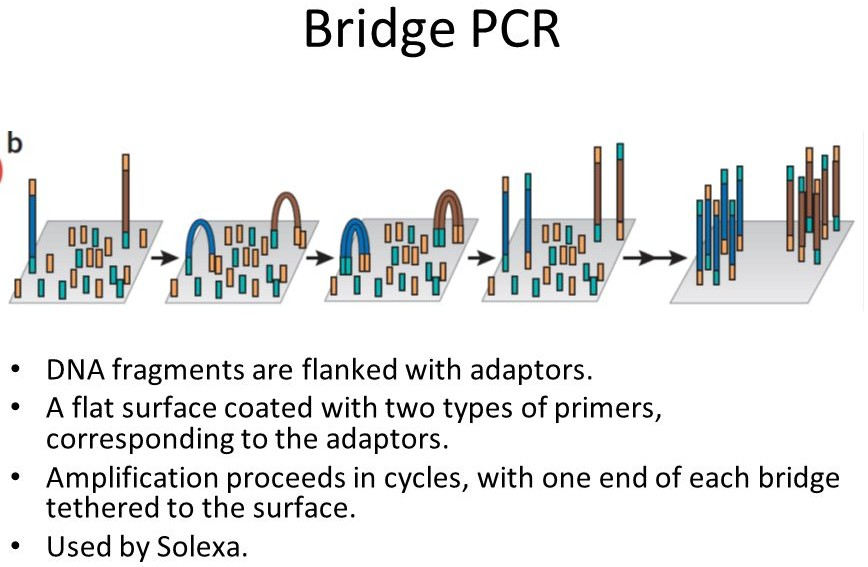
\includegraphics[width=0.9\textwidth]{c2.genomics/sequencing.bridge.01.jpg}
  \end{figure}
\end{frame}

\begin{frame}
  \frametitle{基因组学 | 测序 | 第二代 | 边合成边测序}
  \begin{figure}
    \centering
    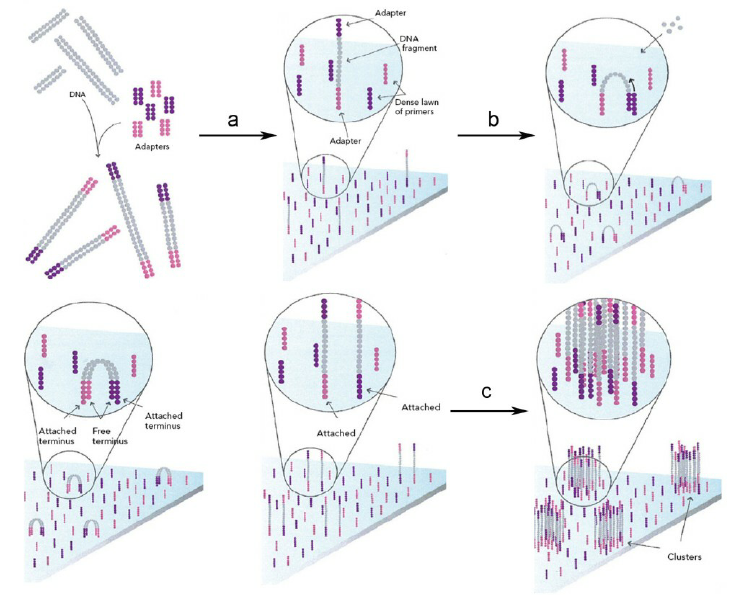
\includegraphics[width=0.8\textwidth]{c2.genomics/sequencing.bridge.02.png}
  \end{figure}
\end{frame}

\begin{frame}
  \frametitle{基因组学 | 测序 | 第二代 | 边合成边测序}
  \begin{figure}
    \centering
    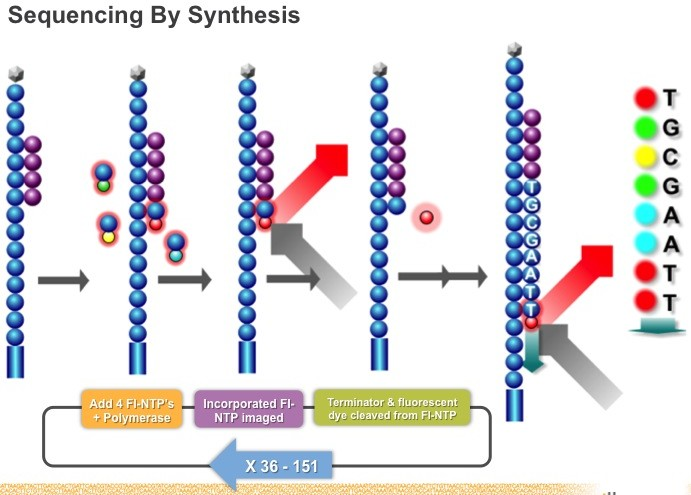
\includegraphics[width=0.9\textwidth]{c2.genomics/sequencing.sbs.01.jpg}
  \end{figure}
\end{frame}

\begin{frame}
  \frametitle{基因组学 | 测序 | 第二代 | 边合成边测序}
  \begin{figure}
    \centering
    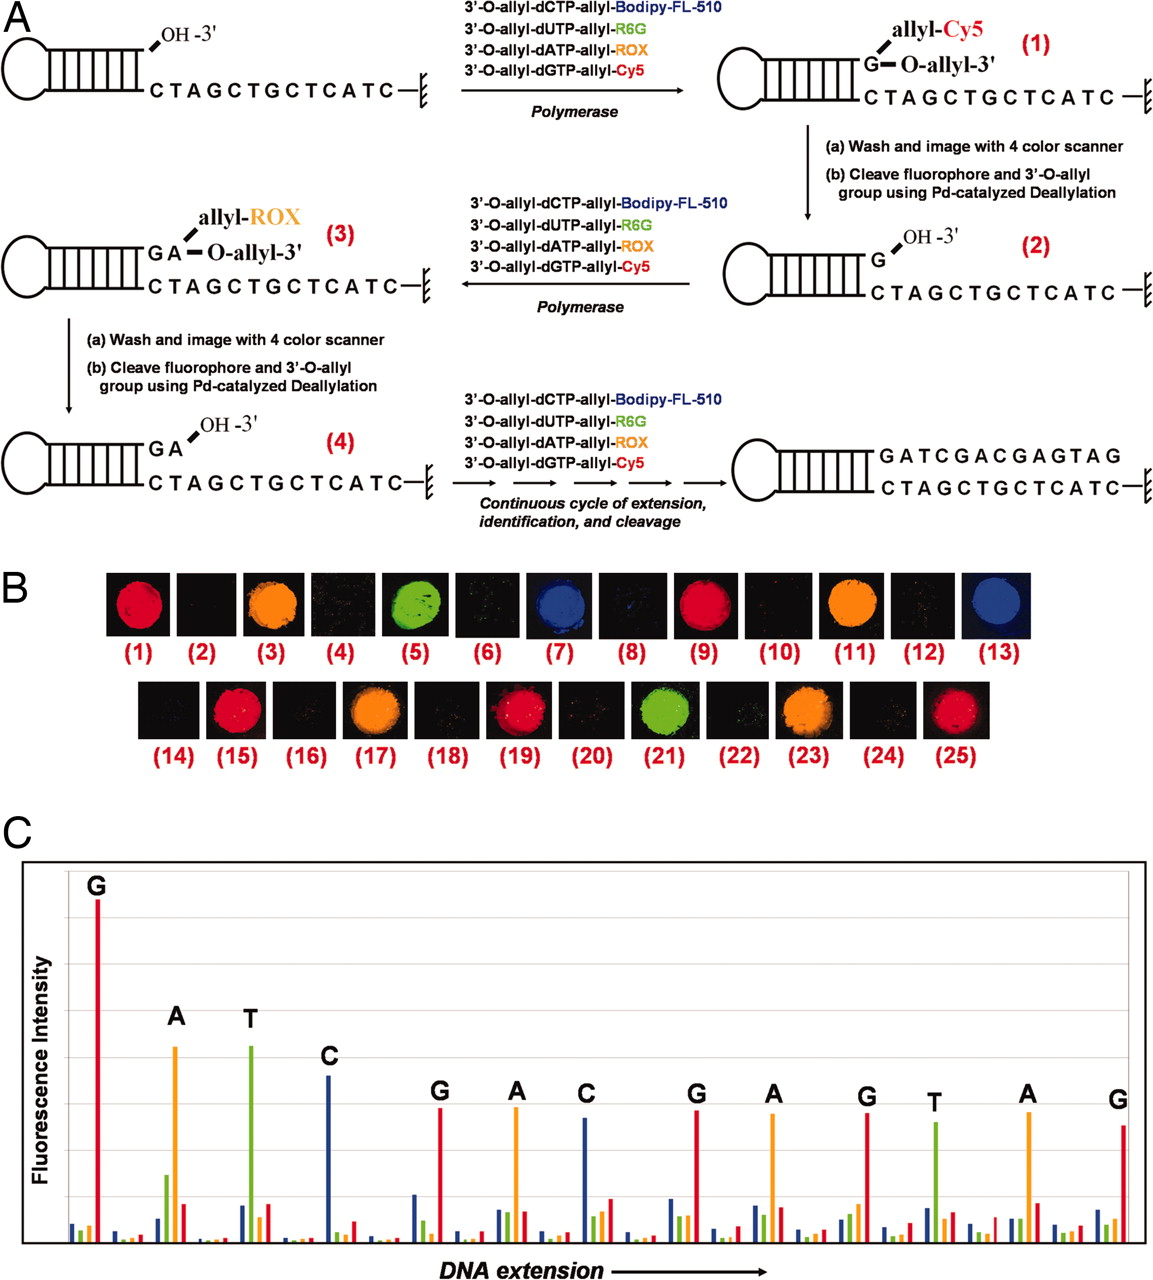
\includegraphics[width=0.59\textwidth]{c2.genomics/sequencing.sbs.04.jpg}
  \end{figure}
\end{frame}

\begin{frame}
  \frametitle{基因组学 | 测序 | 第二代 | 边合成边测序}
  \begin{figure}
    \centering
    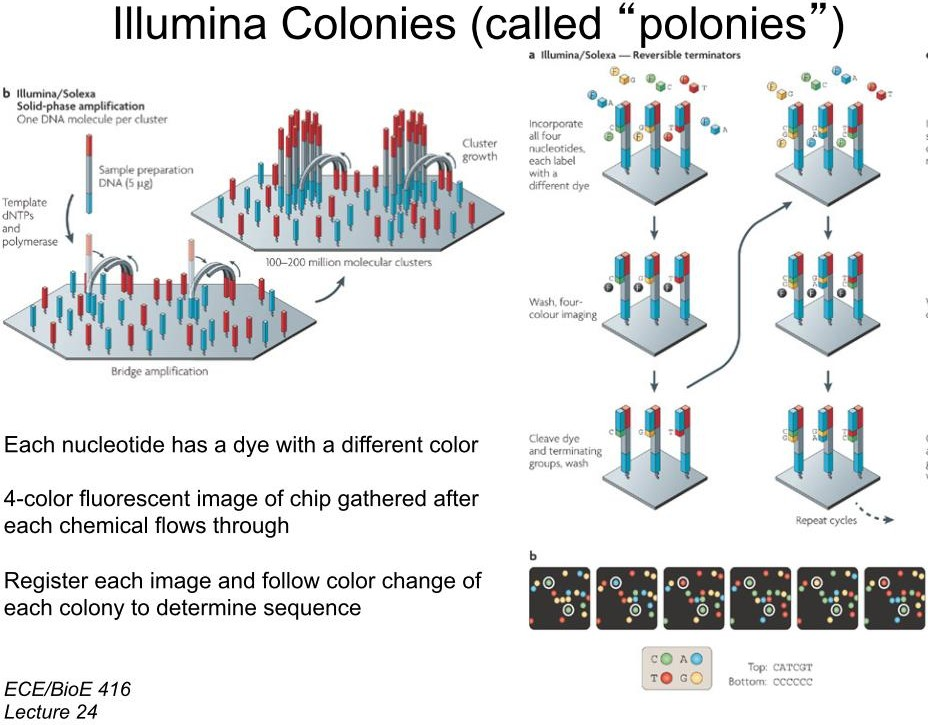
\includegraphics[width=0.82\textwidth]{c2.genomics/sequencing.ill.05.jpg}
  \end{figure}
\end{frame}

\begin{frame}
  \frametitle{基因组学 | 测序 | 第二代 | 边合成边测序}
  \begin{figure}
    \centering
    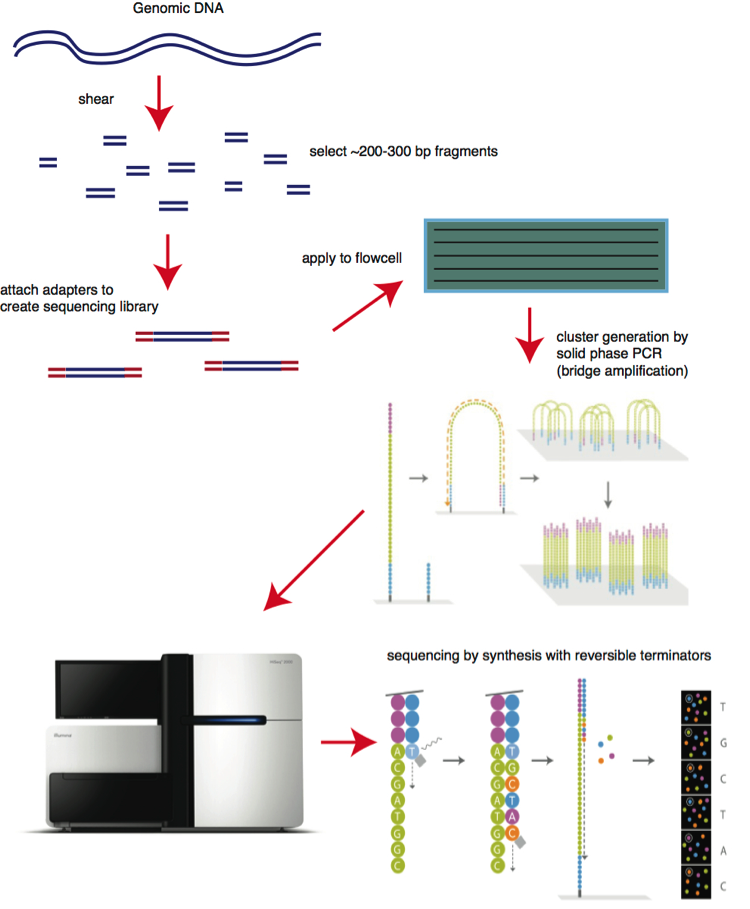
\includegraphics[width=0.52\textwidth]{c2.genomics/sequencing.ill.01.png}
  \end{figure}
\end{frame}

\begin{frame}[label=current]
  \frametitle{基因组学 | 测序 | 第二代 | 边连接边测序}
\end{frame}

\begin{frame}[label=current]
  \frametitle{基因组学 | 测序 | 第二代 | 边连接边测序}
\end{frame}

\begin{frame}[label=current]
  \frametitle{基因组学 | 测序 | 第二代 | 边连接边测序}
\end{frame}

\begin{frame}[label=current]
  \frametitle{基因组学 | 测序 | 第二代 | 边连接边测序}
\end{frame}

\begin{frame}
  \frametitle{基因组学 | 测序 | 第二代 | 总结}
  \begin{figure}
    \centering
    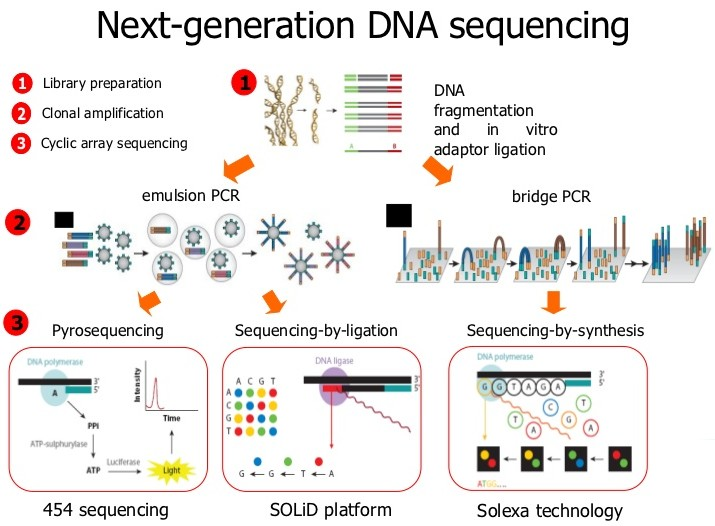
\includegraphics[width=0.9\textwidth]{c2.genomics/sequencing.ngs.01.jpg}
  \end{figure}
\end{frame}

\subsection{第三代测序技术}
\begin{frame}[label=current]
  \frametitle{基因组学 | 测序 | 第三代 | 简介}
\end{frame}

\begin{frame}[label=current]
  \frametitle{基因组学 | 测序 | 第三代 | 离子半导体}
\end{frame}

\begin{frame}[label=current]
  \frametitle{基因组学 | 测序 | 第三代 | 离子半导体}
\end{frame}

\begin{frame}[label=current]
  \frametitle{基因组学 | 测序 | 第三代 | 离子半导体}
\end{frame}

\begin{frame}[label=current]
  \frametitle{基因组学 | 测序 | 第三代 | 单分子实时测序}
\end{frame}

\begin{frame}[label=current]
  \frametitle{基因组学 | 测序 | 第三代 | 单分子实时测序}
\end{frame}

\begin{frame}[label=current]
  \frametitle{基因组学 | 测序 | 第三代 | 单分子实时测序}
\end{frame}

\begin{frame}[label=current]
  \frametitle{基因组学 | 测序 | 第三代 | 单分子实时测序}
\end{frame}

\subsection{测序技术比较}
\begin{frame}
  \frametitle{基因组学 | 测序 | 比较}
  \begin{figure}
    \centering
    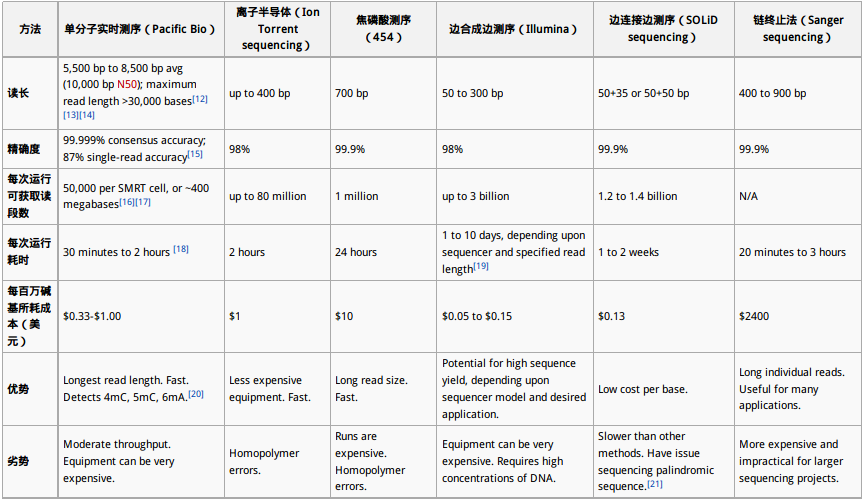
\includegraphics[width=\textwidth]{c2.genomics/sequencing.compare.01.png}
  \end{figure}
\end{frame}

\begin{frame}
  \frametitle{基因组学 | 测序 | 比较}
  \begin{figure}
    \centering
    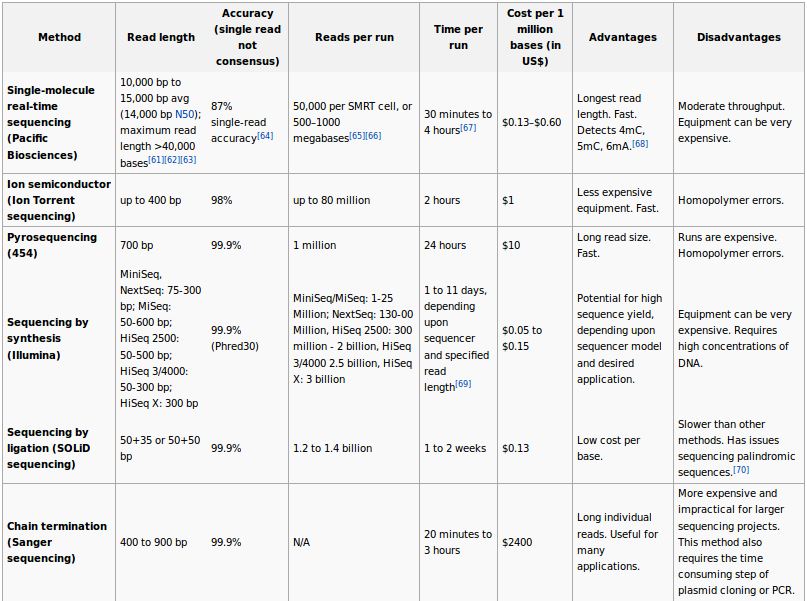
\includegraphics[width=0.85\textwidth]{c2.genomics/sequencing.compare.02.png}
  \end{figure}
\end{frame}

